\documentclass[12pt]{article}

\usepackage[
    a4paper,
    hmargin=2cm, vmargin=1.3cm,
    headheight=56.6pt, % as per the warning by fancyhdr
    headsep=10pt,
    includehead, includefoot
]{geometry}

\usepackage[english]{babel}
\usepackage[utf8x]{inputenc}
\usepackage[T1]{fontenc}

\usepackage{fancyhdr} % extensice control of page headers and footers
\usepackage{graphicx}
\usepackage{parskip} % add space between paragraphs and remove first line's indent
\usepackage[dvipsnames,table]{xcolor} % color the text for the color code: https://en.wikibooks.org/wiki/LaTeX/Colors
\usepackage[bottom]{footmisc} % to place footnotes to the bottom of the page
\usepackage{pdfpages} % \includepdf[pages=-]{myfile.pdf}: all pages, or `pages={1}`
\usepackage{amsmath} % provides math environments
\usepackage{amssymb} % add math symbols
\usepackage{cancel} % https://tex.stackexchange.com/a/75530/164820
\usepackage{ifthen} % provides \ifthenelse test
\usepackage{xifthen} % provides \isempty test
\usepackage{float} % improve the figure placement in the document
\usepackage[normalem]{ulem} % used to strike through: https://jansoehlke.com/2010/06/strikethrough-in-latex/
\usepackage{multirow}
\usepackage{hhline} % https://tex.stackexchange.com/a/39766/164820
% \usepackage[acronym,nonumberlist,nogroupskip]{glossaries} % to handle acronyms

% Fix non breakable links: https://tex.stackexchange.com/a/3034/164820
\PassOptionsToPackage{hyphens}{url}\usepackage{hyperref}
\usepackage[inline]{enumitem} % allow to set some margin to list env's

\usepackage{listings}
\usepackage{tikz}
\usetikzlibrary{calc}
\usepackage{pgfplots}

% ---------------- SETUP HEADER & FOOTER ----------------------
\pagestyle{fancy}
% \fancyhf{} % sets both header and footer to nothing
% \renewcommand{\headrulewidth}{0pt} % remove headers bottom line


% Define variables
\makeatletter
\newcommand{\prof}[1]{\def\@prof{#1}}
\newcommand{\theprof}{\@ifundefined{@prof}{}{\\Prof.: \@prof}}
\newcommand{\student}[1]{\def\@student{#1}}
\newcommand{\thestudent}{\@ifundefined{@student}{}{\@student}}
\newcommand{\seriesnumber}[1]{\def\@seriesnumber{#1}}
\newcommand{\theseriesnumber}{\@ifundefined{@seriesnumber}{}{Series \@seriesnumber}}
\makeatother



\newcommand{\unilogo}[1][0.16\textwidth]{
\includegraphics[width=#1]{logo_uni}}
\newcommand{\mcslogo}[1][0.16\textwidth]{
\includegraphics[width=#1]{logo_mcs}}

\newcommand*{\fullref}[1]{\hyperref[{#1}]{\autoref*{#1}} \textit{\nameref*{#1}}} % https://tex.stackexchange.com/a/121871
\newcommand*{\simpleref}[1]{\hyperref[{#1}]{{\autoref*{#1}}}}
\newcommand*{\namedref}[2]{\hyperref[{#1}]{\textit{#2}}}
\newcommand*{\visitedurl}[2]{\url{#1}\hspace{0.6em}(visited on #2)}
\newcommand*{\footnotelink}[2]{\footnote{\visitedurl{#1}{#2}}}
\newcommand*{\footnotetextlink}[2]{\footnotetext{\visitedurl{#1}{#2}}}


\newcommand{\yellowInBlue}[1]{{\colorbox{blue!50}{\color{yellow}\textbf{#1}}}}

\newcommand*{\todo}[1]{
    \ifthenelse{\isempty{#1}}
        {\yellowInBlue{TODO}}
        {\yellowInBlue{TODO #1}} % else
}



\newcounter{question}[section]
\newcommand{\questioncolor}{\color{CadetBlue}}
\def\newquestion#1{%
    \refstepcounter{question}%
    \textbf{\thequestion. #1}}
\def\question#1{%
    {%
        \questioncolor%
        #1
    }
}


\setlist[description]{leftmargin=0.5cm,labelindent=0.5cm,parsep=0.4ex}


% \glsenablehyper
\hypersetup{
	colorlinks = true,
	% linkcolor = red,
	% menucolor = red,
	% filecolor = blue,
	% anchorcolor = green,
	% urlcolor = blue,
	allcolors = MidnightBlue,
	linkbordercolor = white
}


% \loadglsentries{glossary}
% \makeglossaries


\graphicspath{{assets/}}


\title{
    % \vspace{-2cm}
    \mcslogo[0.3\textwidth]\\[0.9cm]
    Applied Optimization\\
    Exercise 1 - Convex Sets
}
\student{
    V. Carrel \& J. Fontana \& A. Schaller%\\
    % \texttt{20-209-151} \& \texttt{07-406-341} \& \texttt{16-896-375}
}
\prof{Prof. David Bommes}

\seriesnumber{1}
\author{\thestudent\theprof}

\lhead{\unilogo}
\rhead{\thestudent\\\theseriesnumber}


% \usepgfplotslibrary{fillbetween}
\pgfplotsset{compat=newest}
% \usepackage{fontawesome}

\raggedbottom % To avoid stretching the items to fill a page
% ---------------------- DOCUMENT ----------------------------
\begin{document}


\maketitle

%
% Convex Sets
% ---------------------------------
\section{Convex Sets}

\newquestion{Example sets}

\question{Sketch the following sets in $R^2$}
\begin{enumerate}
    \questioncolor
    \item $\displaystyle \text{span}\left\{\binom{1}{1}, \binom{-0.5}{-0.5} \right\} $ \normalcolor

    \begin{figure}[H]
        \center
    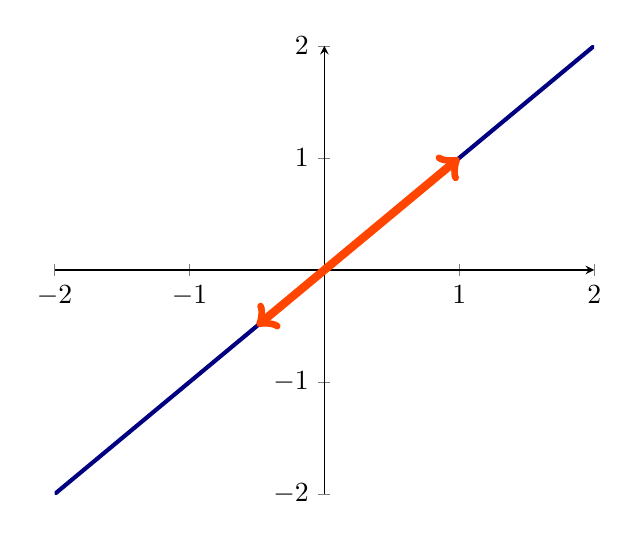
\begin{tikzpicture}
    \begin{axis}[
        %width=0.4\textwidth,
        axis lines=middle,
        xmax=2,
        ymax=2,
        xmin=-2,
        ymin=-2,
        % xlabel={$p_1$},
        % ylabel={$p_2$}
    ]
        \addplot[NavyBlue,samples=2,domain=-2:2,fill opacity=0.05,line width=1.5pt] {x};
        \draw[->, line width=3pt, color=OrangeRed] (0,0) -- (1,1);
        \draw[->, line width=3pt, color=OrangeRed] (0,0) -- (-0.5,-0.5);
    \end{axis}
    \end{tikzpicture}

    \end{figure}


    \pagebreak
    \questioncolor
    \item $\displaystyle \text{span}\left\{\binom{1}{1}, \binom{0.5}{-0.5} \right\} $ \normalcolor


    \begin{figure}[H]
        \center
    \begin{tikzpicture}
    \begin{axis}[
        %width=0.4\textwidth,
        axis lines=middle,
        xmax=2,
        ymax=2,
        xmin=-2,
        ymin=-2,
        % xlabel={$p_1$},
        % ylabel={$p_2$}
    ]
        \draw[pattern=north west lines, pattern color=NavyBlue,fill opacity=0.7] (-2.1,-2.1) rectangle (4.1,4.1);
        \draw[->, line width=3pt, color=OrangeRed] (0,0) -- (1,1);
        \draw[->, line width=3pt, color=OrangeRed] (0,0) -- (0.5,-0.5);
    \end{axis}
    \end{tikzpicture}

    \end{figure}


    \questioncolor
    \item $\displaystyle \text{aff}\left\{\binom{1}{0}, \binom{1}{-1} \right\} $ \normalcolor



    \begin{figure}[H]
        \center
    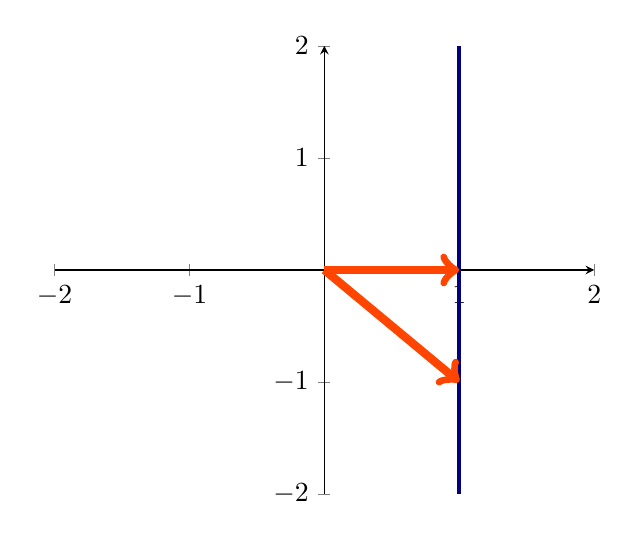
\begin{tikzpicture}
    \begin{axis}[
        %width=0.4\textwidth,
        axis lines=middle,
        xmax=2,
        ymax=2,
        xmin=-2,
        ymin=-2,
        % xlabel={$p_1$},
        % ylabel={$p_2$}
    ]
        \draw[color=NavyBlue,fill opacity=0.7,line width=1.5pt] (1,-2) -- (1,2);
        \draw[->, line width=3pt, color=OrangeRed] (0,0) -- (1,0);
        \draw[->, line width=3pt, color=OrangeRed] (0,0) -- (1,-1);
    \end{axis}
    \end{tikzpicture}

    \end{figure}


    \pagebreak
    \questioncolor
    \item $\displaystyle \text{conv}\left\{\binom{1}{0}, \binom{2}{1}, \binom{3}{-2}, \binom{-1}{0}, \binom{-2}{1}, \binom{-2}{-2} \right\} $ \normalcolor


    \begin{figure}[H]
        \center
    \begin{tikzpicture}
    \begin{axis}[
        %width=0.4\textwidth,
        axis lines=middle,
        xmax=4,
        ymax=2,
        xmin=-3,
        ymin=-3,
        % xlabel={$p_1$},
        % ylabel={$p_2$}
    ]
        \draw[pattern=north west lines, pattern color=NavyBlue,color=NavyBlue,fill opacity=0.7,line width=1.5pt]
        (2,1) --
        (3,-2) --
        (-2,-2) --
        (-2,1) --
        cycle;
        \draw[OrangeRed,fill]
            (1,0) circle [radius=3pt]
            (2,1) circle [radius=3pt]
            (3,-2) circle [radius=3pt]
            (-1,0) circle [radius=3pt]
            (-2,1) circle [radius=3pt]
            (-2,-2) circle [radius=3pt];
    \end{axis}
    \end{tikzpicture}

    \end{figure}


\end{enumerate}


\bigskip
\bigskip
\newquestion{Convexity}

\question{Let $C \in R^n$ be a convex set, with $x_1,...,x_k \in C$, and let $\theta_1,...,\theta_k \in R$ satisfy $\theta_i \ge 0$,$\theta_1 + ... + \theta_k = 1$. Show that $\theta_1 x_1 + ... + \theta_k x_k \in C$. (The definition of convexity is that this holds for $k = 2$; you must show it for arbitrary $k$.) Hint. Use induction on $k$.}

\emph{Show.} that $\theta_1 + ... + \theta_k \in C$

\begin{proof}

    \underline{Base Case $k = 2$} By definition, it holds for $k = 2$.

    \underline{Inductive Step} Assume it is correct for $k = n$, then for $k = n + 1$, we have:
    $$x_1,...,x_{n+1} \in C$$
    $$\theta_1,...,\theta_{n+1} \in C$$
    with $\theta_i \ge 0$ and $\sum\limits_{i=0}^{n+1} \theta_i = 1 \Rightarrow \theta_{n+1} = 1 - \sum\limits_{i=1}^{n} \theta_i$
    $$\Rightarrow \sum_{i=1}^{n+1} \theta_i x_i = \sum_{i=1}^{n} \theta_i x_i + \theta_{n+1} x_{n+1} = \sum_{i=1}^{n} \theta_i x_i + x_{n+1} = \sum_{i=1}^{n} \theta_i x_{n+1}$$%
    $$= \underbrace{x_{n+1}}_\text{$\in C$} \underbrace{\sum_{i=1}^{n} \theta_i (x_i - x_{n+1})}_{\substack{\text{$\in C$ by hypothesis on $k=n$} \\ \text{because $\sum\limits_{i=1}^{n}\theta_i \in [0,1]$}}} \Biggr\} \Rightarrow \in C $$

\end{proof}



\newquestion{Linear Equations}

\question{Show that the solution set of linear equations $\{x | Ax = b\}$ with $x \in R^n$, $A \in R^{m×n}$ and $b \in R^m$ is an affine set.}

\begin{proof}
    Let $x_0, x_1$ be solutions of linear equations, i.e. $A x_0 = b$ and $A x_1 = b$

    Then $$A((1-\beta)x_0 + \beta x_1) = (1-\beta) A x_0 + \beta A x_1$$$$ = (1-\beta)b + \beta b = b$$

    $\Rightarrow$ The set is affine.
\end{proof}



\bigskip
\bigskip
\newquestion{Linear Inequations}

\begin{enumerate}
    \questioncolor
    \item Show that the solution set of linear inequations $\{x | Ax \preceq b, Cx = d\}$ with $x \in R^n$, $A \in R^{m×n}$ and $b \in R^m$, $C \in R^{k×n}$ and $d \in R^k$ is a convex set. Here $\preceq$ means componentwise less or equal. \normalcolor

    \begin{proof}
        Let $x_0, x_1$ be solutions of linear inequations, i.e. $A x_0 \preceq b, C x_0 = d$ and $A x_1 \preceq b, C x_1 = d$, for $\beta \in [0, 1]$

        Then
        \begin{equation}\label{eq:eq1}
            A((1-\beta)x_0 + \beta x_1) = \underbrace{(1-\beta)}_\text{$\ge 0$} \underbrace{A x_0}_\text{$\preceq b$} + \underbrace{\beta}_\text{$\ge 0$} \underbrace{A x_1}_\text{$\preceq b$} \preceq (1-\beta) b + \beta b = b
        \end{equation}

        and $$C((1-\beta) x_0 + \beta x_1) = (1-\beta) C x_0 + \beta C x_1 = (1-\beta) d + \beta d = d$$

        $\Rightarrow$ convex set.
    \end{proof}



    \questioncolor
    \item Is it an affine set? \normalcolor

    No, cf \simpleref{eq:eq1}, if we don't have the $a_i \ge 0$ for $\forall i$ constraint, it removes the constraint on the $\beta \in [0,1]$, which then means we could have $(1-\beta) < 0$. Therefore the step $(1-\beta)Ax_0 \le b$ is not doable, we might have $(1-\beta)Ax_0 \ge b$\hfill $\blacksquare$
\end{enumerate}




\pagebreak
\newquestion{Voronoi description of halfspace}

\question{Let $a$ and $b$ be distinct points in $R^n$. Show that the set of all points that are closer (in Euclidean norm) to $a$ than $b$, i.e., $\{x | \left\lVert x − a\right\rVert ^2 \le \left\lVert x − b\right\rVert ^2\}$, is a halfspace. Describe it explicitly as an inequality of the form $c^T x \le d$. Draw a picture.}

\begin{proof}
Be $c \in R^n$ a vector, $c = b - a$ be $d \in R$, $d=c^T x_0 = c^T \frac{a+b}{2}$

then we have the halfspace $$\left\{x \bigg| (b-a)^T x \le \frac{(b-a)^T(b-a)}{2}\right\} $$
\end{proof}

\emph{Check.} $$\left\lVert x-a \right\rVert^2 \le \left\lVert x-b \right\rVert^2$$$$\Leftrightarrow (x-a)^T(x-a) \le (x-b)^T(x-b)$$$$\Leftrightarrow \cancel{x^Tx} -2a^Tx+a^Ta \le \cancel{x^Tx}-2b^Tx + b^Tb$$$$\Leftrightarrow (b-a)^T x \le (b^Tb-a^Ta)\ \frac{1}{2}$$

\begin{figure}[H]
    \center
    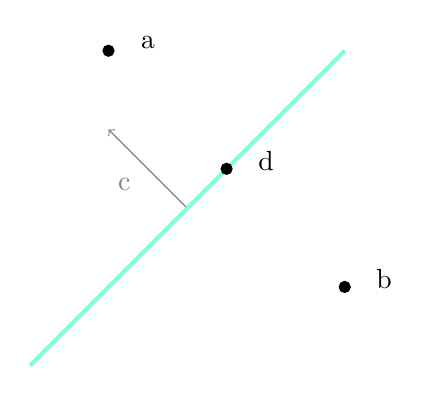
\begin{tikzpicture}
        \draw[->,color=gray] (0,0) -- (-1,1);
        \node[color=gray] at (-0.8,0.3){c};

        \draw[color=Aquamarine,line width=1.5pt] (-2,-2) -- (2,2);

        \draw[fill]
        (-1,2) circle [radius=2pt]
        (0.5,0.5) circle [radius=2pt]
        (2,-1) circle [radius=2pt];

        \begin{scope}[shift={(0.5,0.1)}]
            \node at (-1,2){a};
            \node at (0.5,0.5){d};
            \node at (2,-1){b};
        \end{scope}
    \end{tikzpicture}
\end{figure}







%
% Convex Illumination Problem
% ---------------------------------
\pagebreak
\section{Convex Illumination Problem}

\question{Show that the solution $p^∗ =(p_1^∗,p_2^∗,...,p_∗^n)^T \in R^n$ of the non-convex illumination problem from the lecture
\begin{align*}
    \text{minimize}&\quad \max\limits_{k=1...m} \big| \log I_k - \log I_{des} \big|\\
    \text{subject to}&\quad 0 \le p_j \le p_{max}, \quad j=1...n
\end{align*}
with $I_k =\sum\limits_{j = 1}^{n} a_{kj} p_j$ for geometric constants $a_{jk} \in R$, a constant desired illumination $I_{des} \in R$ and an upper bound $p_{max} \in R$ on the lamp power, is identical to the solution of the following equivalent (convex) problem
\begin{align*}
    \text{minimize}&\quad \max\limits_{k=1...m} h(I_k / I_{des})\\
    \text{subject to}&\quad 0 \le p_j \le p_{max}, \quad j=1...n
\end{align*}
with $h(u) = max\{u, \frac{1}{u}\}$.}


\begin{proof}
    \begin{alignat*}{2}
        \max_{k=1,...,m}& \big| \log(I_k) - \log(I_{des}) \big|
        \quad&& \Big|\ \text{log rules}\\%
%
        &= \max_{k=1,...,m} \Bigg| \log \bigg( \frac{I_k}{I_{des}} \bigg) \Bigg|
        \quad&& \Big|\ \text{remove | . |}\\%
%
        &= \max_{k=1,...,m} \max \Bigg\{ \log \bigg( \frac{I_k}{I_{des}} \bigg), \log \bigg( \frac{I_{des}}{I_k} \bigg) \Bigg\}
        \quad&& \Big|\ \text{max log = log max}\\%
%
        &= \log \max_{k=1,...,m} \max \Bigg\{  \frac{I_k}{I_{des}} , \frac{I_{des}}{I_k} \Bigg\}
        \quad&& \Big|\ \text{with}\ h=(u) = max \bigg\{u, \frac{1}{u}\bigg\}\\%
%
        &= \log \max_{k=1,...,m} h \bigg( \frac{I_k}{I_{des}} \bigg)
    \end{alignat*}

The $\log$ is a monotonically increasing function, i.e. $\forall x, y$ with $x \le y$ we have $\log(x) \le \log(y)$.\\
So when minimizing, we can remove it without affecting the solution.

$\Rightarrow = \max_{k=1,...,m} h \bigg( \frac{I_k}{I_{des}} \bigg)$ with $h(u) = \max \bigg\{ u, \frac{1}{u} \bigg\}$.
\end{proof}


\end{document}